%!TEX root = ../reports.tex
%
% 固体の比熱
% レポート用紙
%

\stepcounter{section}
\section*{固体の比熱}

\begin{center}
\begin{tabular}{|c|c|c|c|}
\hline
\parbox[c][1.2cm][c]{0cm}{}学籍番号 & \hspace{3cm} & 名前 & \hspace{6cm} \\
\hline
\parbox[c][1.2cm][c]{0cm}{}実験日時 & \multicolumn{3}{|l|}{   年  月  日  曜日  時限}\\
\hline
\parbox[c][2.0cm][c]{0cm}{}共同実験者 & \multicolumn{3}{|l|}{}\\
\hline
\end{tabular}
\end{center}

\subsection*{実験の目的}

\vspace{4cm}

\subsection*{測定値および計算}

\subjikken{}

\subsubsection*{実験前測定}

銅製容器およびかくはん器(ツマミを取り外したもの)の合計質量
\[
M' = \hspace{4cm} \text{[g]}
\]

\bigskip

\hspace*{-\parindent}
\begin{tabular}{|l|p{3.5cm}|p{3.5cm}|p{3.5cm}|}
\hline
 & 試料A & 試料B & 試料C \\
\hline
試料の色や特徴 & & & \\
(予想される材質) & & & \\
\hline
試料の質量 $m$ [g] & & & \\
\hline
容器中の水の質量 $M$ [g] & & & \\
\hline
\end{tabular}

 \newpage


\subsubsection*{温度測定}



\hspace*{-\parindent}
\begin{tabular}{|c|c||c|c||c|c|}
\hline
\multicolumn{2}{|l||}{試料A} & \multicolumn{2}{|l||}{試料B} & \multicolumn{2}{|l|}{試料C} \\
\hline
時間 [秒] & 水温 [℃] & 時間 [秒] & 水温  [℃] & 時間 [秒] & 水温  [℃] \\
\hline
\hspace*{2cm}&\hspace*{2cm}&\hspace*{2cm}&\hspace*{2cm}&\hspace*{2cm}&\hspace*{2cm}\\
\hline
&&&&&\\
\hline
&&&&&\\
\hline
&&&&&\\
\hline
&&&&&\\
\hline
&&&&&\\
\hline
&&&&&\\
\hline
&&&&&\\
\hline
&&&&&\\
\hline
&&&&&\\
\hline
\end{tabular}

%\subsubsection*{プロット}
%\bigskip\bigskip
%\hspace*{-\parindent}
%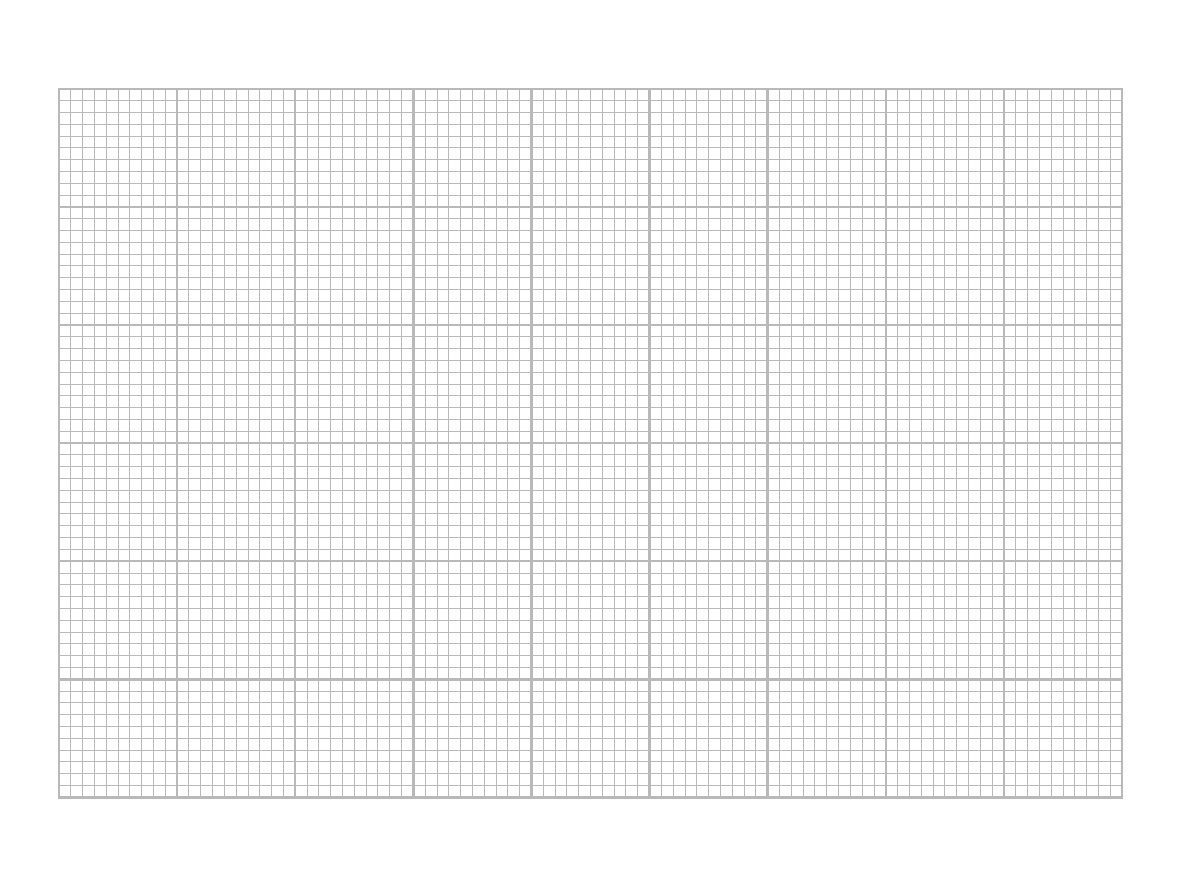
\includegraphics[scale=0.93]{FranckHertz/graph.pdf}

%\newpage

\bigskip

\hspace*{-\parindent}
\begin{tabular}{|l|p{3.5cm}|p{3.5cm}|p{3.5cm}|}
\hline
 & 試料A & 試料B & 試料C \\
\hline
最初の試料温度 $T_1$ [℃] & & & \\
\hline
最初の水温 $T_2$ [℃] & & & \\
\hline
最終温度 $T_3$ [℃] & & & \\
\hline
\end{tabular}


\subsubsection*{比熱の計算}
\[
C = \frac{(M C_W+M'C') (T_3-T_2)}{m (T_1-T_3) } \,\,  \text{[J/gK]}
\qquad
(C_W = 4.2\,\,\text{[J/gK]}, \quad C' = 0.38\,\,\text{[J/gK]})
\]
\hspace*{-\parindent}
\begin{tabular}{|l|p{4cm}|p{4cm}|p{4cm}|}
\hline
 & 試料A & 試料B & 試料C \\
\hline
比熱 $C$ [J/gK] & & & \\
\hline
\end{tabular}

\newpage

\subsection*{考察}

\begin{itemize}

\item 求めた比熱を比較検討し、それぞれの資料の材質を同定してみましょう。

\vspace{6cm}

\item 比熱の大小はどのような意味を持つか、考察してみましょう。

\vspace{6cm}

\item 比熱の違い(性質)に関連した身の回りの現象や応用例について調べてみましょう。


\end{itemize}
